\section{LoRa module}
In order to test the LoRa SX1278 module, one wrote a small program to test send and receive functions from LoRa module, with the usage shown in figure \ref{fig:loratest}.

\begin{figure}[H]
	\centering	
	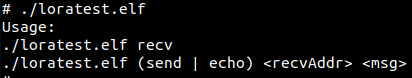
\includegraphics[width=0.6\textwidth]{13tests/lora/loratest}
	\caption{Test LoRa module.}
	\label{fig:loratest}
\end{figure}

Using two LoRa modules, one was connected to a Raspberry Pi in\linebreak
\verb|tomas-abreu|'s computer with local address defined as \verb|0xbb|, the other was connected to another Raspberry Pi in \verb|fernandes|'s computer with local address \verb|0xcc|.

One tested the read and send functions of the module, firstly by waiting for a message, as shown in figure \ref{fig:loratest_recv}.

\begin{figure}[H]
	\centering	
	\includegraphics[width=0.6\textwidth]{13tests/lora/BB_recv_wait}
	\caption{Test LoRa module: waiting for receive.}
	\label{fig:loratest_recv}
\end{figure}

In figure \ref{fig:loratest_send} (a) the device \verb|0xcc| sends the message \verb|"Hello from 0xCC"| to the device \verb|0xbb|, presenting all the attributes, from the source address, \verb|'from'| field, to the destination address, \verb|'to'| field, including also message attributes, as the \verb|msgID|, \verb|msgLength| and the \verb|msg| itself.

In figure \ref{fig:loratest_send} (b) is shown the receiver side, receiving the message correctly, with error 0, and presenting all the attributes from the received message, matching all that were sent by the sender.

\begin{figure}[H]%
	\centering
	\subfloat[\centering Sender side ]{{\includegraphics[width=6.25cm]{13tests/lora/CC_send}}}%
	\qquad
	\subfloat[\centering Receiver side ]{{\includegraphics[width=6.25cm]{13tests/lora/BB_recv}}}%
	\caption{Test LoRa module: send message from 0xcc to 0xbb.}%
	\label{fig:loratest_send}%
\end{figure}
	
As previously seen, the SPI interface works by sending two bytes in a row, depending on what operation it is: read or write. In figure \ref{fig:loratest_sck_nss} is seen the clock signal (SCK, in red) and the slave select signal (NSS, in yellow).

\begin{figure}[H]
	\centering	
	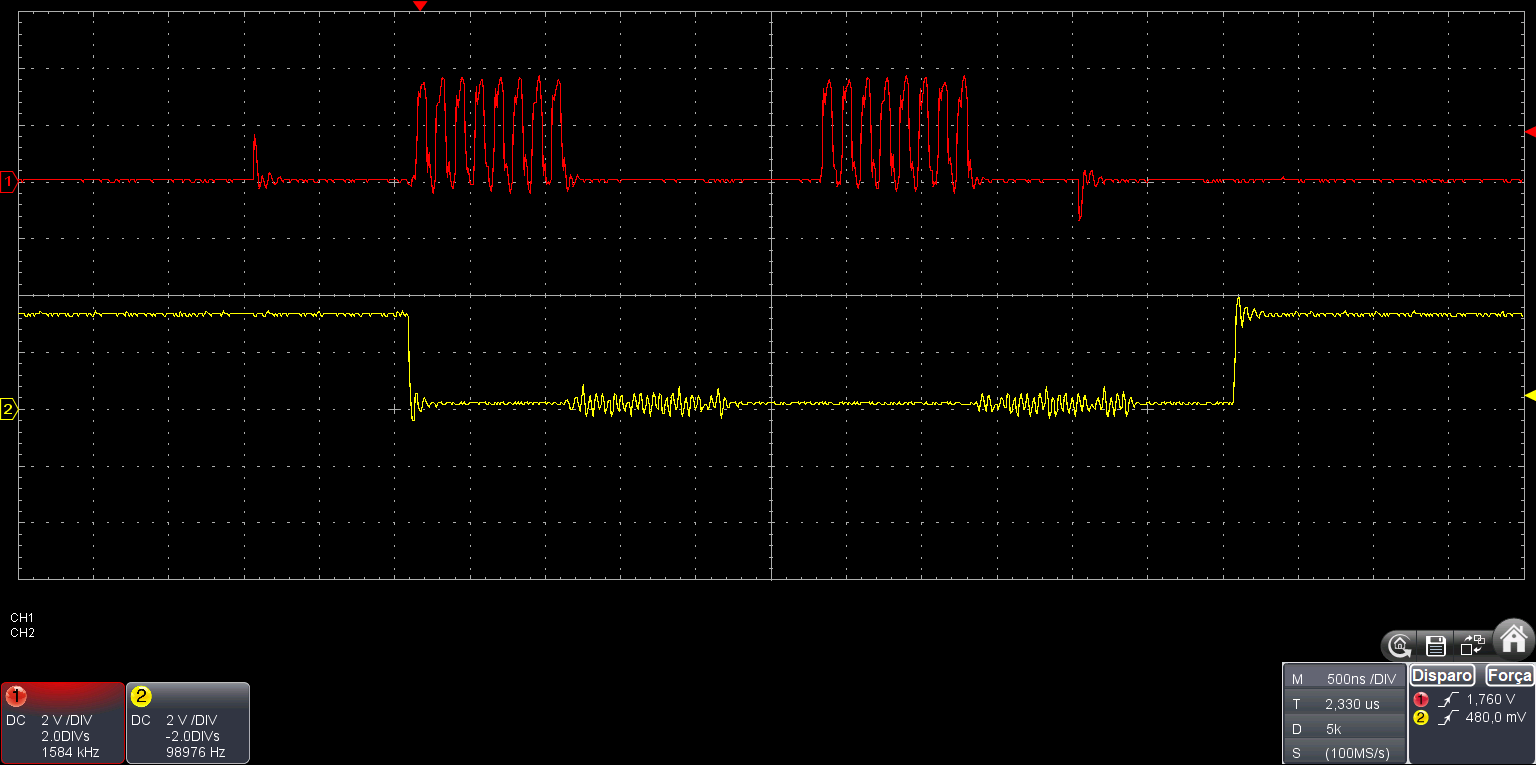
\includegraphics[width=1\textwidth]{13tests/lora/SCK_CS}
	\caption{Test LoRa module: SCK (in red) and NSS (in yellow) signals.}
	\label{fig:loratest_sck_nss}
\end{figure}

When the NSS goes to low, a transfer is started, with the master generating SCK. For each byte are generated 8 pulses of clock, 1 pulse per bit sent. Due to overhead and delays introduced by the software, there is a gap between the two bytes sent, where the NSS signal is still low but the SCK is not being generated. When NSS goes high, the transfer is over.

%**********************************************************
\section{TSL2581}
After the I2C configuration, one can see that the TSL2581 was detected in the bus by the Raspberry Pi, by running the command \verb|i2cdetect -y 1|. The execution of this command detects all the devices connected to the I2C bus and, as seen in the figure \ref{fig:i2cDetect}, it detects the TSL2581 device with its default address, 0x39, as seen before \ref{section:lumSensor}. One can also see what type of operations are allowed to this device, by running the command \verb|i2cdetect -F 1|.

\begin{figure}[H]
	\centering	
	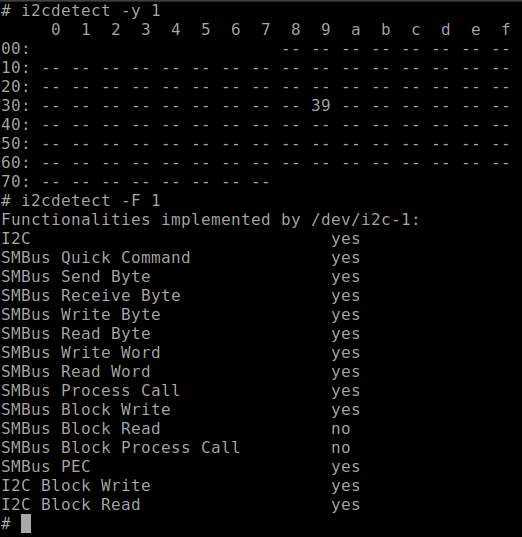
\includegraphics[width=.6\textwidth]{13tests/ldr/i2c_detect}
	\caption{Test TSL2581 module: device detection in I2C bus.}
	\label{fig:i2cDetect}
\end{figure}

After the device was detected in the I2C bus, one wrote a small program to test the values read by the sensor module. The figure \ref{fig:testtsl} shows the execution of the test program, \verb|testtsl.elf|, that prints the values read from the sensor every second.

\begin{figure}[H]
	\centering	
	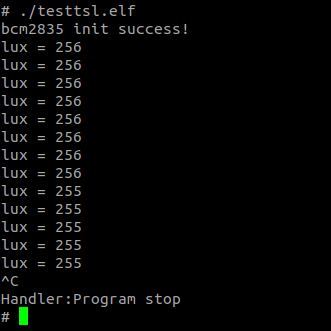
\includegraphics[width=.5\textwidth]{13tests/ldr/testtsl}
	\caption{Test TSL2581 module: Test program for TSL2581.}
	\label{fig:testtsl}
\end{figure}

As previously seen, the I2C communication protocol uses a clock line and a data line. The communications start by the master sending the slave address to the bus, and if the correspondent slave responds, then the master can send other commands to the slave. In figure \ref{fig:i2c_SCL_SDA} is presented the clock line (SCL), in red, and the data line (SDA), in yellow, and shows that in the first eight bits of clock, the master sends the slave address \verb|0x39|. In the next eight bits of clock, the master sends a command to read the low byte of the \textit{Channel\_0}, being the command sent by the master equal to \verb|0xD4|.

\begin{figure}[H]
	\centering	
	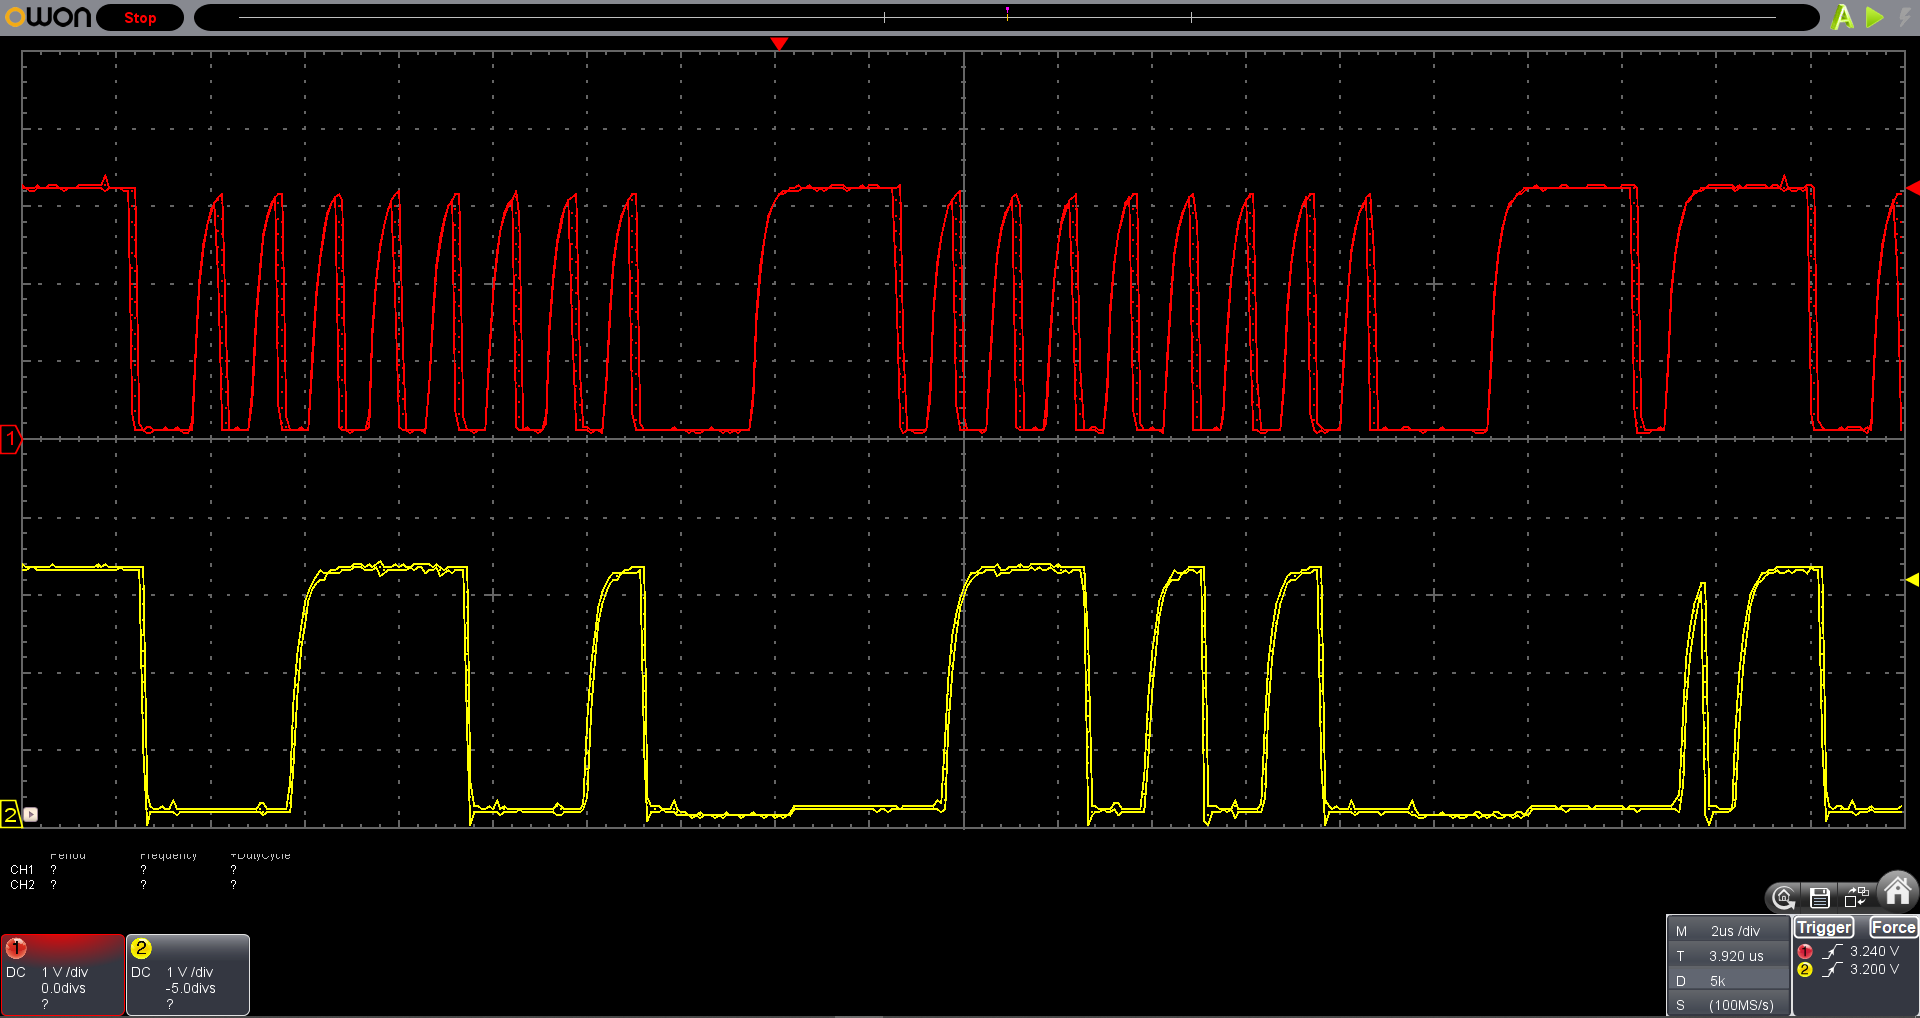
\includegraphics[width=1\textwidth]{13tests/ldr/scl_sda_i2c}
	\caption{Test TSL2581 module: Transmission of two bytes: SCL (in red) and SCK (in yellow) signals.}
	\label{fig:i2c_SCL_SDA}
\end{figure}

The figure \ref{fig:tsl} shows the montage of the TSL2581 with the Raspberry Pi, with the interrupt pin not being used.

\begin{figure}[H]
	\centering	
	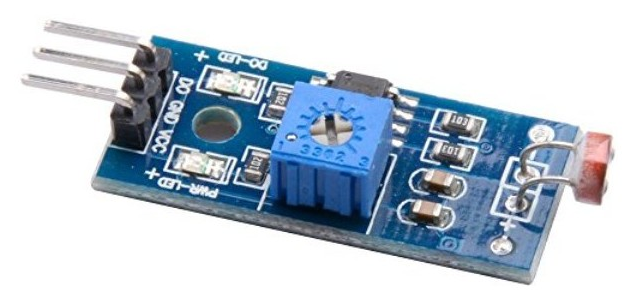
\includegraphics[width=.9\textwidth]{13tests/ldr/ldr}
	\caption{Test TSL2581 module: Montage.}
	\label{fig:tsl}
\end{figure}

%**********************************************************
\section{PWM control}
In order to test PWM control, one wrote a small program to test the generation of a PWM signal at 50 Hz with a variable duty cycle, with the usage shown in figure \ref{fig:loratest}. The duty cycle received is a value from 0 to 1.

\begin{figure}[H]
	\centering	
	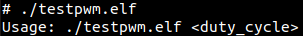
\includegraphics[width=.5\textwidth]{13tests/pwm/testpwm}
	\caption{Test PWM control.}
	\label{fig:testpwm}
\end{figure}

In figure \ref{fig:pwm_50} one defined duty cycle as \verb|0,5| (\verb+50 %+). As seen in the Implementation phase, the \verb+RANGE = 67500+ , so considering the inserted duty cycle, the PWM pulse ratio should be \verb|RANGE*0,5 = 33750|, as shown in figure \ref{fig:pwm_50} (a), in the field \verb|PWM data|.

In figure \ref{fig:pwm_50} (b) is shown the generated PWM signal, with time division of \verb+5 ms+ per division, adding up to \verb+20 ms+ per period, which is referent to a 50 Hz wave.

\begin{figure}[H]%
	\centering
	\subfloat[\centering Set duty cycle to 50\%. ]{{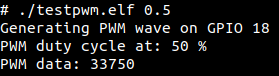
\includegraphics[width=6.25cm]{13tests/pwm/pwm_50}}}%
	\qquad
	\subfloat[\centering Generated PWM signal. ]{{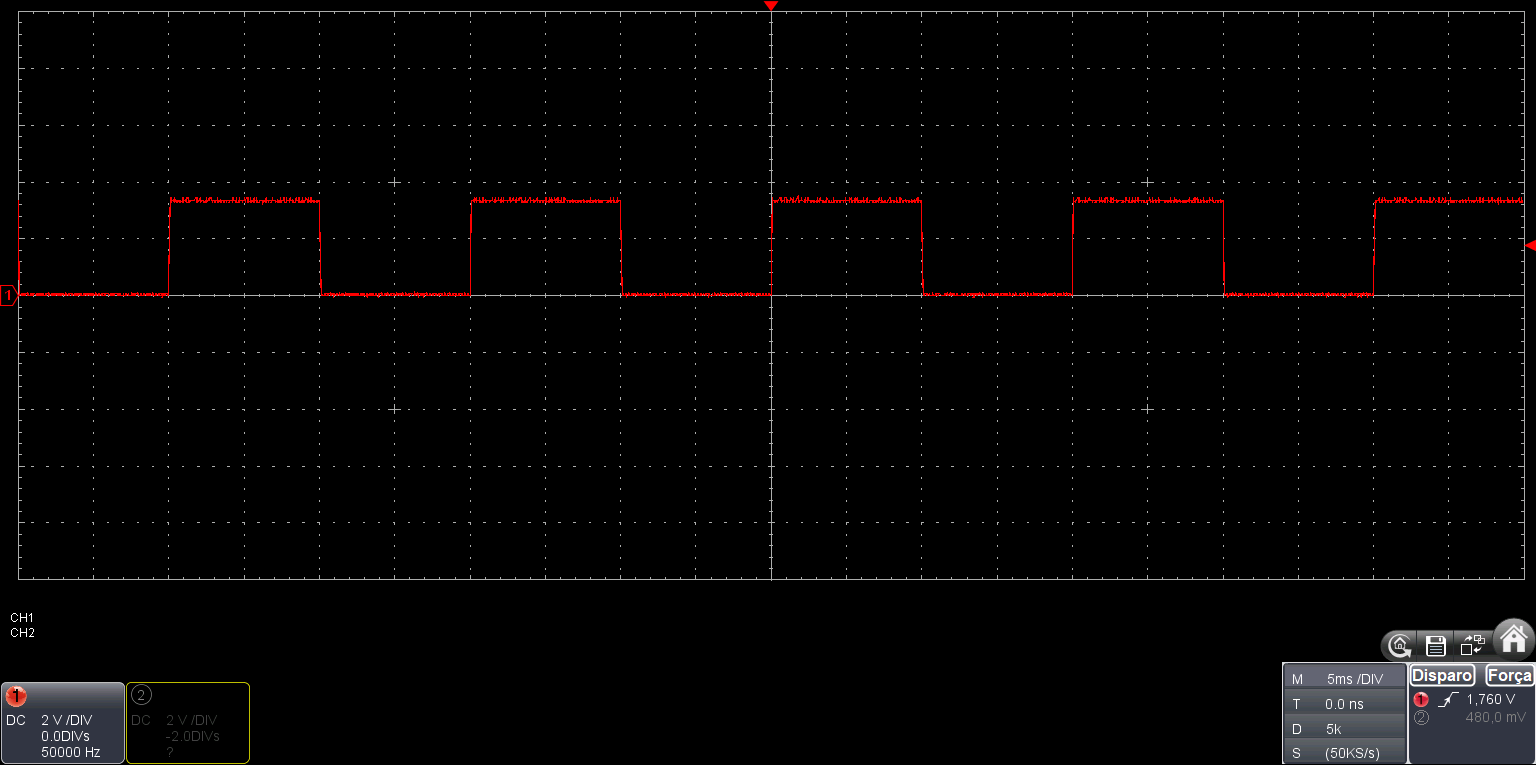
\includegraphics[width=12cm]{13tests/pwm/Duty_50}}}%
	\caption{Test PWM control: PWM at 50\% duty cycle.}%
	\label{fig:pwm_50}%
\end{figure}

In figure \ref{fig:pwm_25} is shown the a PWM generated signal with \verb+25 %+ duty cycle, with output on the GPIO 18. In figure \ref{fig:pwm_25} (a) one can check that the field \verb|PWM data| is equal to \verb+RANGE*0,25+.

\begin{figure}[H]%
	\centering
	\subfloat[\centering Set duty cycle to 25\%. ]{{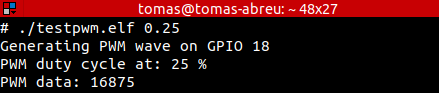
\includegraphics[width=6.25cm]{13tests/pwm/pwm_25}}}%
	\qquad
	\subfloat[\centering Generated PWM signal. ]{{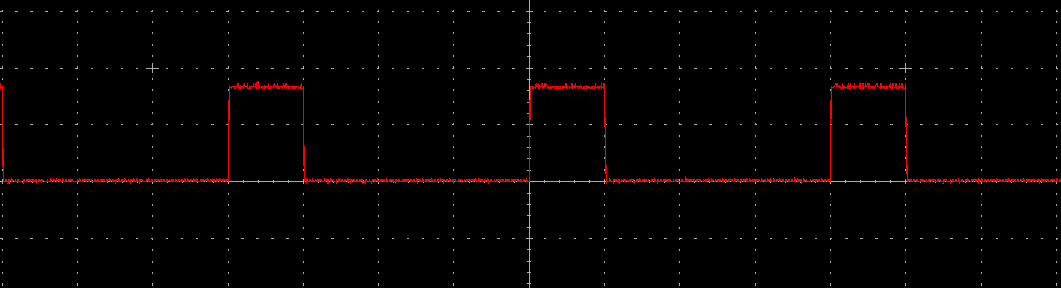
\includegraphics[width=12cm]{13tests/pwm/Duty_25}}}%
	\caption{Test PWM control: PWM at 25\% duty cycle.}%
	\label{fig:pwm_25}%
\end{figure}

%**********************************************************
\section{Motion Detector}

As mentioned before, for the motion detector, the PIR HC-SR501, it was implemented a device driver. After insert its module in the kernel using the \verb|insmod| command, one can test if the sensor detects movement, using a small test code. In figure \ref{fig:testpir}, one can see the execution of the program that shows that the sensor detected movement.

\begin{figure}[H]
	\centering	
	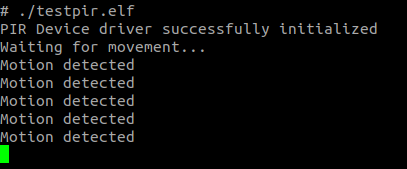
\includegraphics[width=.5\textwidth]{13tests/pir/testpir}
	\caption{Test PIR HC-SR501 module: Detection of movement.}
	\label{fig:testpir}
\end{figure}

In figure \ref{fig:pirMount}, it is shown the the movement sensor connected to the Raspberry Pi. During the tests, it was noticed that the sensor must be stable to not detect false positives. Furthermore, there is a insignificant delay in the detection of the movement, despite the attempts to adjust, using the potentiometers in the module.

\begin{figure}[H]
	\centering	
	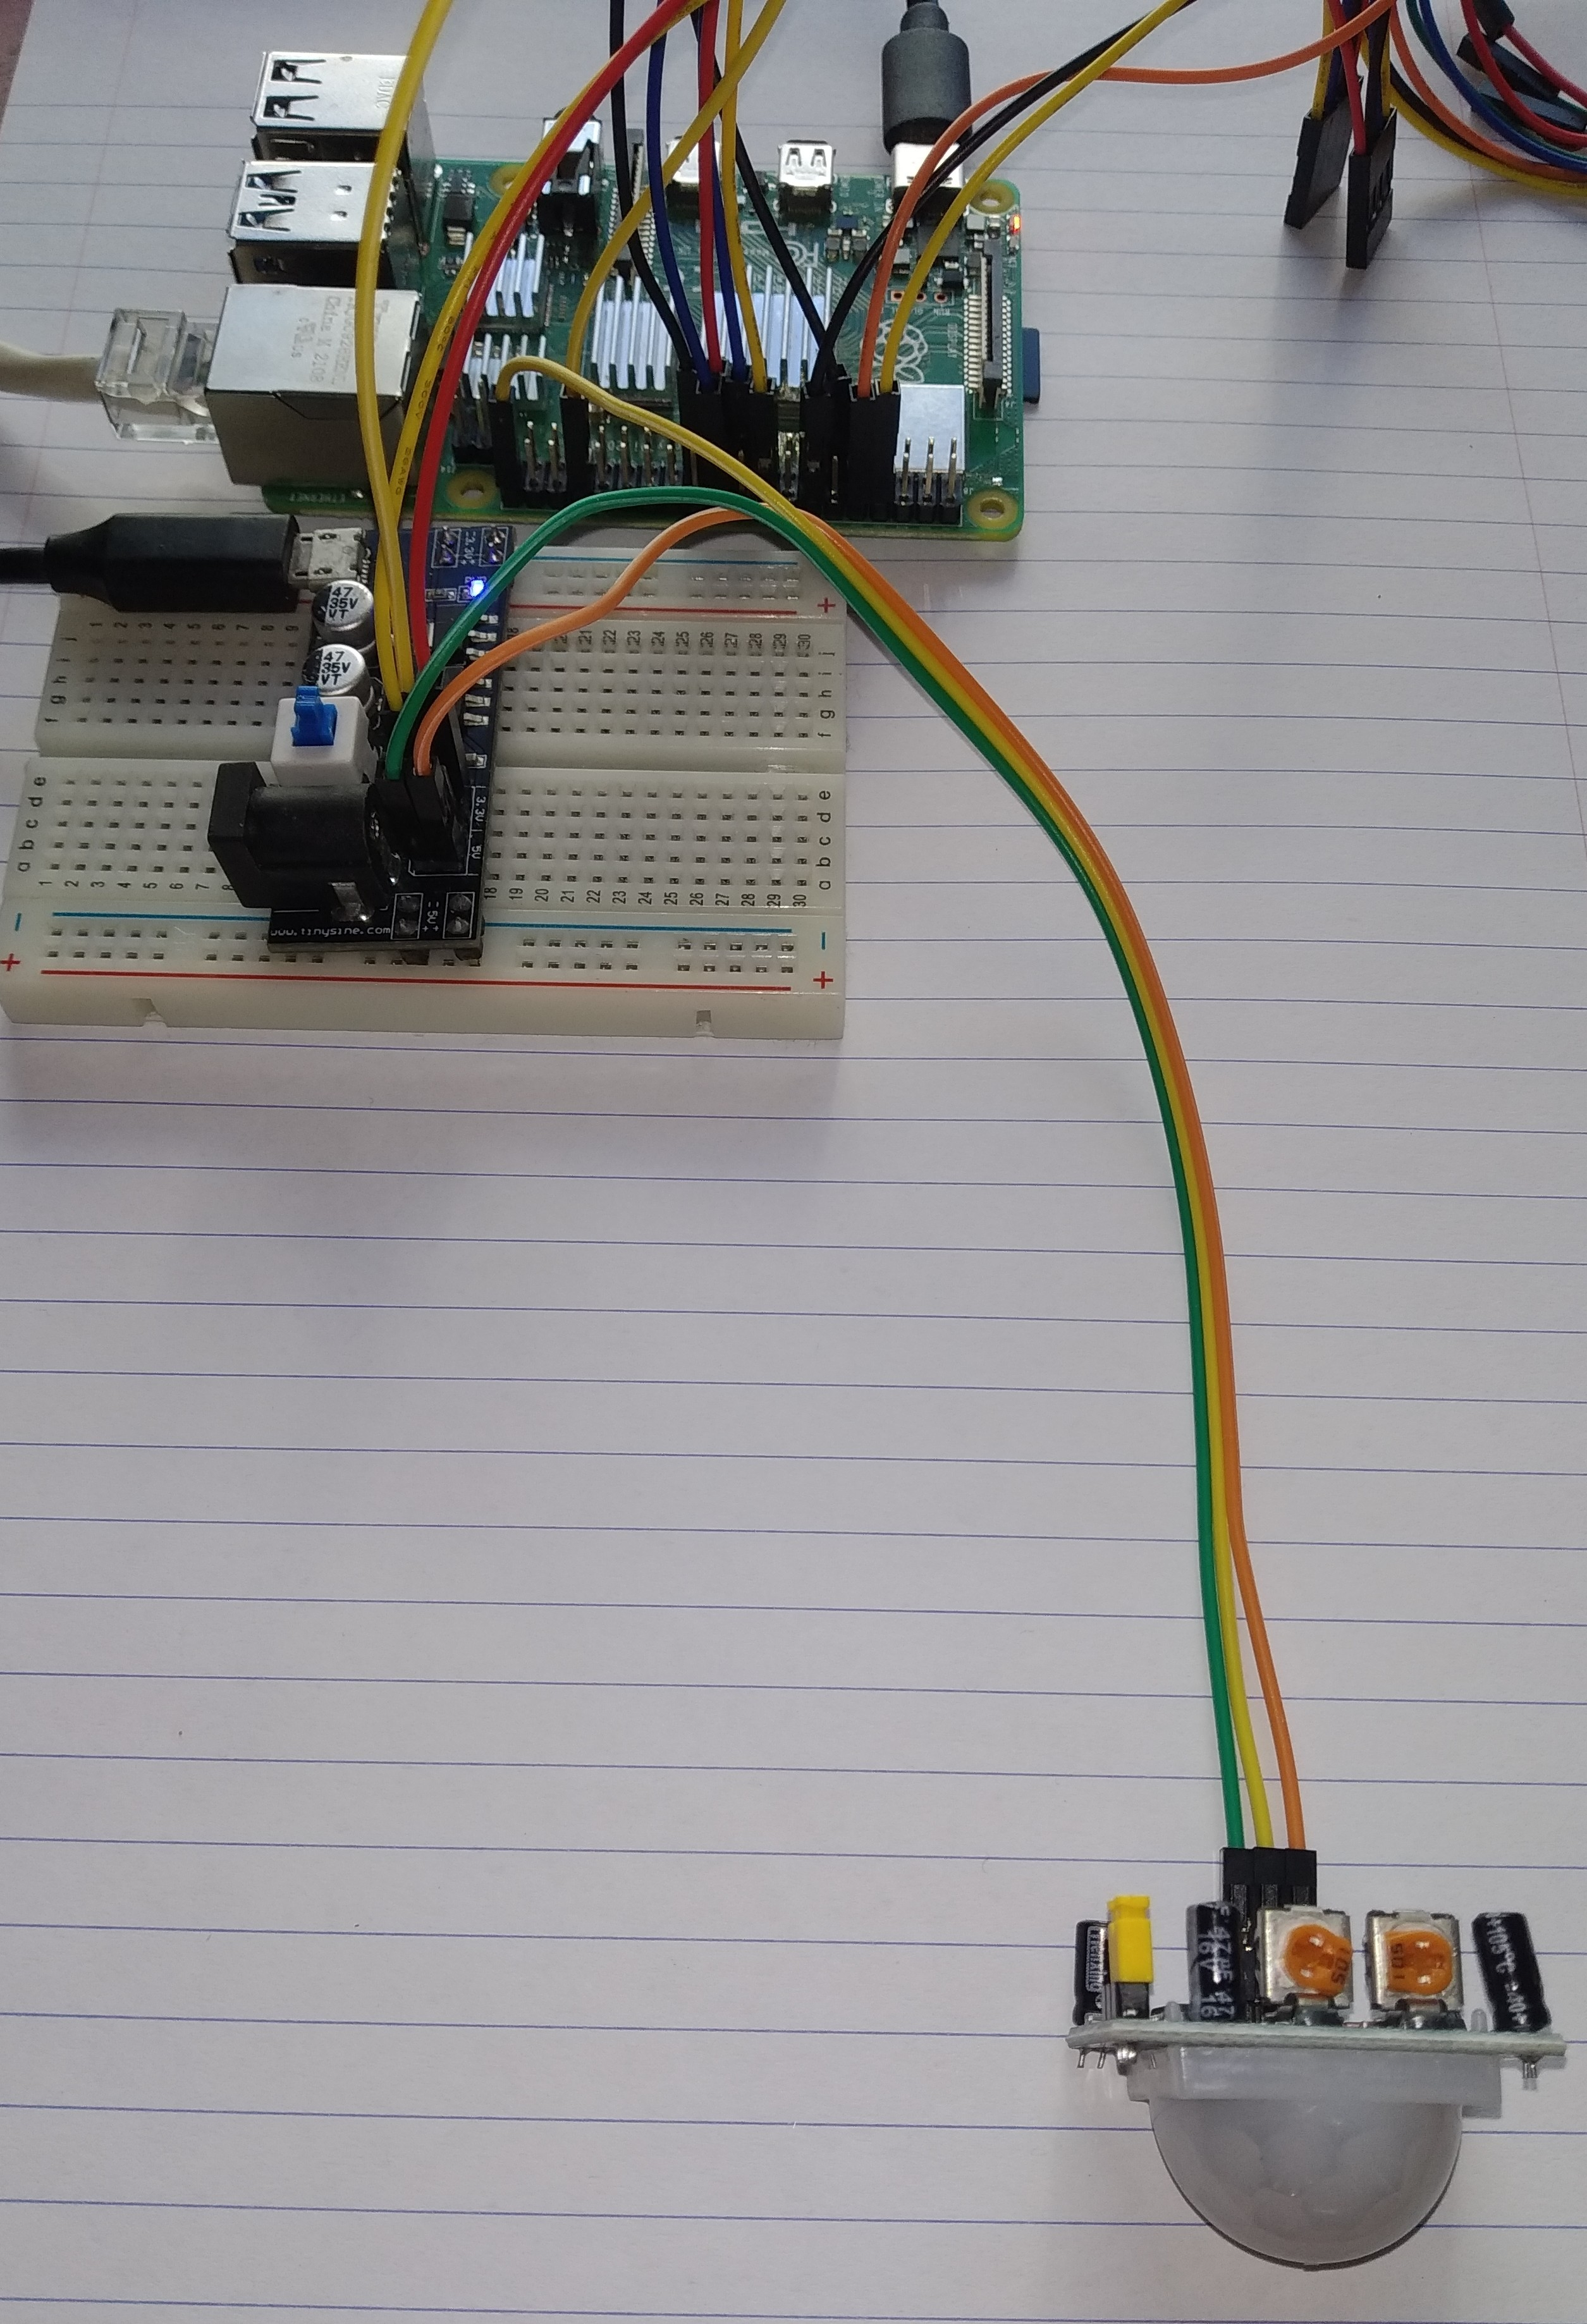
\includegraphics[width=.4\textwidth]{13tests/pir/pir}
	\caption{Test PIR HC-SR501 module: Montage.}
	\label{fig:pirMount}
\end{figure}

%**********************************************************
\section{Lamp Failure Detector}

As seen in the previous chapter, one will use the Lamp Failure Detector to know if the lamp is working or broken. In order to test this sensor, it was developed a small program that reads the sensor in polling mode. In figure \ref{fig:testlampf}, one can see the execution of the program that shows that the sensor detected a failure in the lamp, this is, not detected light.

\begin{figure}[H]
	\centering	
	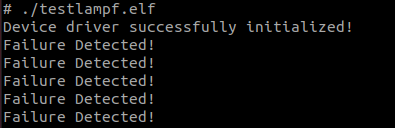
\includegraphics[width=.65\textwidth]{13tests/lampf/testlampf}
	\caption{Test LDR module: Lamp failure detection.}
	\label{fig:testlampf}
\end{figure}

%**********************************************************
\section{Camera}

To know if the camera was detected by the Raspberry Pi, it was used the command \verb|vcgencmd get_camera|, and the result was \verb|supported=1 detected=1|, showing that the camera was successfully detected. Next, it was used a small program to open the camera, take a picture and store it locally. In the figure \ref{fig:firstpic} is shown the first photo taken with the camera and the figure \ref{fig:secpic} shows a photo taken after calibrating the camera values.

\begin{figure}[H]
	\centering
	\begin{subfigure}{.4\textwidth}
		\centering
		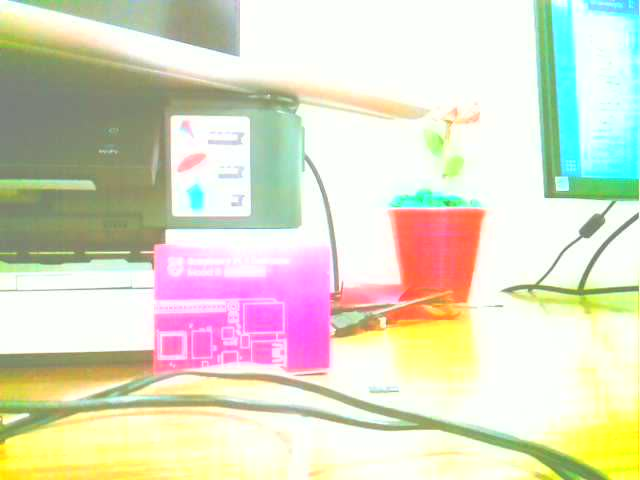
\includegraphics[width=.95\linewidth]{13tests/camera/firstpic}
		\caption{Photo before calibration.}
		\label{fig:firstpic}
	\end{subfigure}%
	\begin{subfigure}{.4\textwidth}
		\centering
		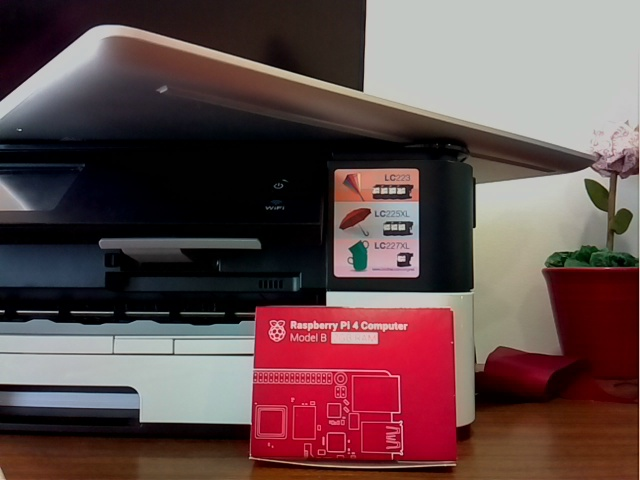
\includegraphics[width=.95\linewidth]{13tests/camera/secpic}
		\caption{Photo after calibration.}
		\label{fig:secpic}
	\end{subfigure}
	\caption{Test Camera.}
	\label{fig:pics}
\end{figure}

%**********************************************************
\section{Parking Spots Detection}

Regarding the parking spots detection, it was done a three phase tests. First, it was tested the algorithm that detects the parking spot outline, next the algorithm that detects cars in an image and, at last, the empty parking spots detection.

In figure \ref{fig:parkoutline} is shown the result of the parking spots outline detection. As one can see, the algorithm detected the rectangles that compose a parking spot.

\begin{figure}[H]
	\centering	
	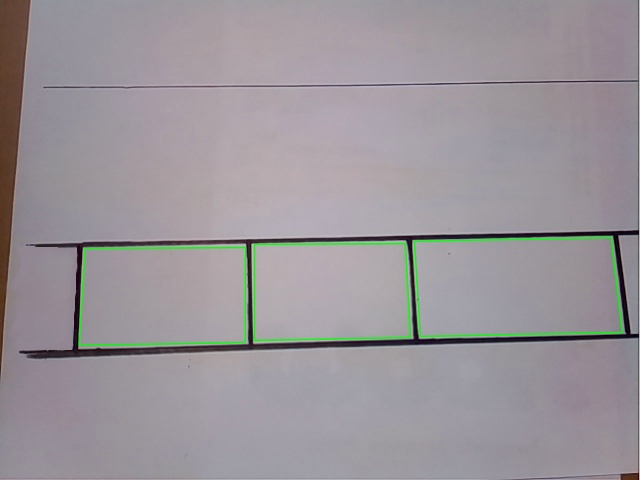
\includegraphics[width=.45\textwidth]{13tests/park/ParkOutline}
	\caption{Test Parking Spots Detection: Parking spot outline.}
	\label{fig:parkoutline}
\end{figure}

Regarding the cars detection, in figure \ref{fig:carsDetect}, one can see that all cars were detected in the image.

\begin{figure}[H]
	\centering	
	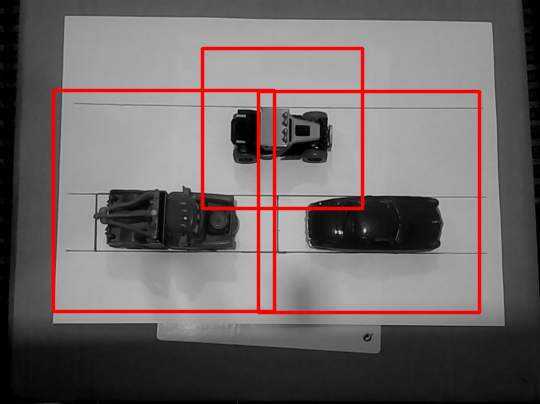
\includegraphics[width=.45\textwidth]{13tests/park/3cars_W}
	\caption{Test Parking Spots Detection: 3 cars detection.}
	\label{fig:carsDetect}
\end{figure}

However, this detection showed some errors, principally when detecting cars near other cars, as reflects the figure \ref{fig:carsNW}, or detecting false positives in the image as observed in figure \ref{fig:0carsNW}. This happens because, to train the classifier, was used a different angle of the cars than in this images. 
%The solution for this problem would be train the haar cascade classifier with other images or use other object detection algorithms, like CNN or YOLO.

\begin{figure}[H]
	\centering
	\begin{subfigure}{.4\textwidth}
		\centering
		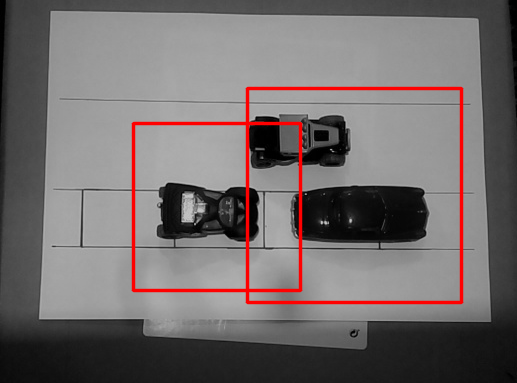
\includegraphics[width=.95\linewidth]{13tests/park/3cars_nw}
		\caption{3 cars detection.}
		\label{fig:carsNW}
	\end{subfigure}%
	\begin{subfigure}{.4\textwidth}
		\centering
		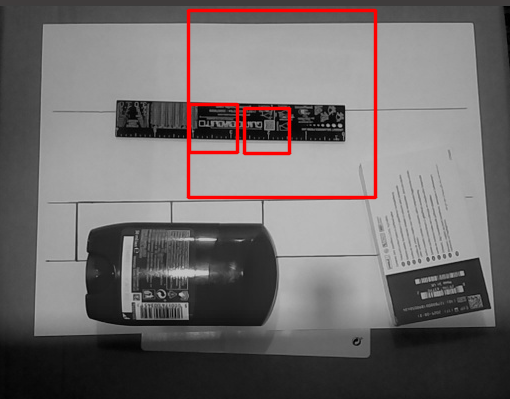
\includegraphics[width=.95\linewidth]{13tests/park/0car_NW}
		\caption{0 cars detection.}
		\label{fig:0carsNW}
	\end{subfigure}
	\caption{Testing Parking Spots Detection: Bad cars detection.}
	\label{fig:cars}
\end{figure}

Finally, one tested the two algorithms together. In figure \ref{fig:2parks}, is shown the detection of two parking spots available, as one car is occupying one parking spot, and, in figure \ref{fig:1park}, can be observed one park detection, as there are two cars occupying parking spots. Note that the the empty parking spots are represented as green rectangles and the occupied parking spots are represented as red rectangles.

\begin{figure}[H]
	\centering
	\begin{subfigure}{.5\textwidth}
		\centering
		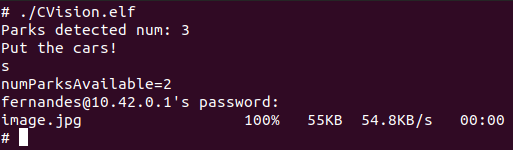
\includegraphics[width=.99\linewidth]{13tests/park/2parks_t}
		\caption{Program execution.}
		\label{fig:2parkst}
	\end{subfigure}%
	\begin{subfigure}{.4\textwidth}
		\centering
		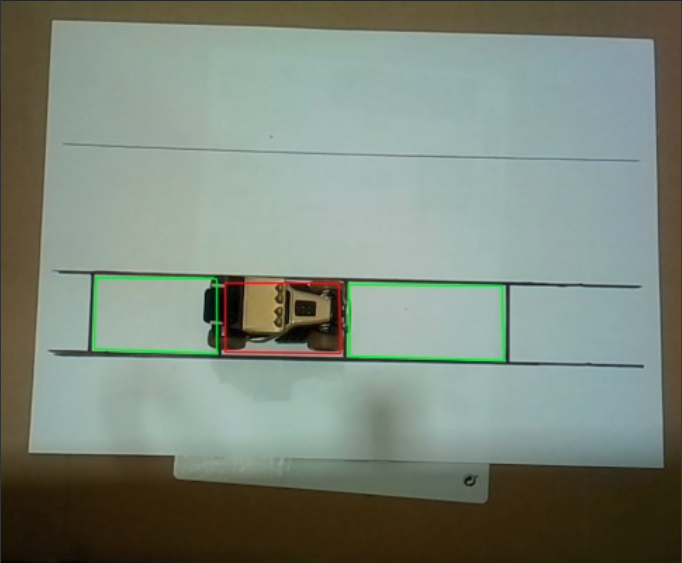
\includegraphics[width=.95\linewidth]{13tests/park/2parks}
		\caption{Detection.}
		\label{fig:2parksim}
	\end{subfigure}
	\caption{Testing Parking Spots Detection: 2 empty parking spots.}
	\label{fig:2parks}
\end{figure}

\begin{figure}[H]
	\centering
	\begin{subfigure}{.5\textwidth}
		\centering
		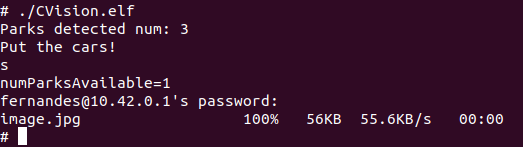
\includegraphics[width=.99\linewidth]{13tests/park/1park_t}
		\caption{Program execution.}
		\label{fig:1parkst}
	\end{subfigure}%
	\begin{subfigure}{.4\textwidth}
		\centering
		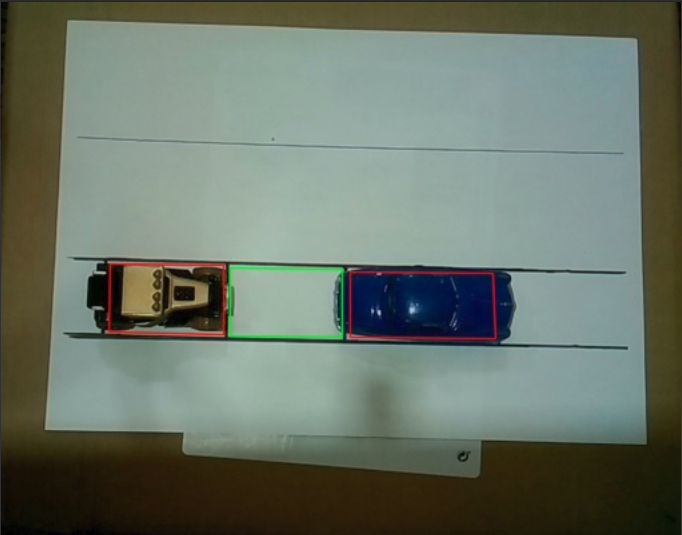
\includegraphics[width=.95\linewidth]{13tests/park/1park}
		\caption{Detection.}
		\label{fig:1parksim}
	\end{subfigure}
	\caption{Testing Parking Spots Detection: 1 empty parking spots.}
	\label{fig:1park}
\end{figure}

One has recorded a video (available on \url{https://www.youtube.com/watch?v=6i_ds_ChGGM}) demonstrating the parking spots detection algorithm tests, already integrated in the local system.

%%**********************************************************
%\section{Database}

%**********************************************************
\section{Local System}
Regarding Local System tests, one recorded a video (available on \linebreak \url{https://youtu.be/DqlRUeHZ5FM}) demonstrating the local system working, with all the modules integrated.

The first tests presented was the parking spots detection algorithms, previously seen in this chapter. The tests for the parking spots detection integrated in the local system are shown in a recorded video (available on \url{https://www.youtube.com/watch?v=6i_ds_ChGGM}). In figure \ref{fig:testpark}, one can see that the algorithm detected 3 parking spots. After putting one car in a parking spot, the local system detected only two parks available and sent it to the remote system. When another car is added to the parking spot, the local system does the same and send the information that there's only one parking spot detected.

\begin{figure}[H]
	\centering	
	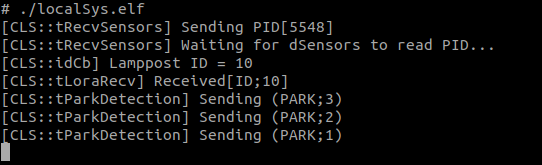
\includegraphics[width=.55\textwidth]{13tests/tParkDetection}
	\caption{Test Local System: Parking spots detection.}
	\label{fig:testpark}
\end{figure}

Next, the video shows all the sensors working. For this tests, one also recorded another video showing the movement detection (available on \url{https://youtu.be/kcBeJNxGR2k}). In figure \ref{fig:localSys}, one can observe the local system tests with the sensors integrated. At first, the local system waits for the sensors daemon to read the PID. When the PID is read, the sensors daemon may start to send commands. When it gets dark, the light sensor, TSL2581, detects low luminosity and the daemon sends a command to the main process to turn on the light at the minimum brightness, \verb|MIN|. If the movement sensor, PIR, sensor detects movement, the daemon sends a command to turn on the light at maximum brightness. The lamp continues at maximum brightness until the lamp timer has a timeout, putting it to the minimum brightness again. If the lamp fails, i.e., the lamp failure detector doesn't detect light, then the daemon send a command, informing the main process that the lamp failed, \verb|FAIL|. At last, if the light sensor detects day time lux values, the daemon sends the command \verb|OFF|, in order to the main process turn off the light. 

\begin{figure}[H]
	\centering
	\begin{subfigure}{.5\textwidth}
		\centering	
		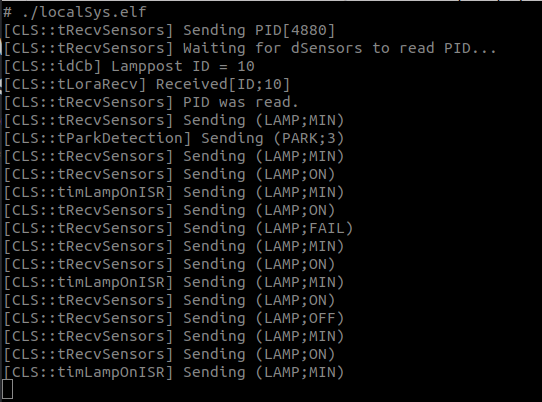
\includegraphics[width=.95\textwidth]{13tests/localSys}
		\caption{Main Process.}
		\label{fig:main}
	\end{subfigure}%
	\begin{subfigure}{.5\textwidth}
		\centering
		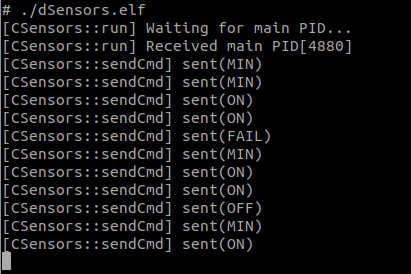
\includegraphics[width=.95\linewidth]{13tests/dSensors}
		\caption{Sensors Daemon.}
		\label{fig:dSensors}
	\end{subfigure}
	\caption{Testing Local System.}
	\label{fig:localSys}
\end{figure}

The local system transmits all the information via LoRa communication to the gateway, if it is connected to him, in order to update the remote system. As one can see in \ref{fig:main}, the data sent to the gateway have the structure \verb|<COMMAND>;<INFO_COMMAND>|. In the next section, one will approach the communication tests in the gateway.

%**********************************************************
\section{Gateway}
The gateway is connected to the remote system through TCP-IP, using an ethernet cable. In this case, when connecting to the remote system, the gateway tries to connect to IP \verb|10.42.0.1|, network address of the remote system which is listening for incoming connections on port \verb|5000|. After TCP connection has been established, the gateway needs to identify himself as a remote client, specifying its type, i.e, \verb|GATEWAY|. This identification is done using \verb|TYPE;<clientType>| command.

\begin{figure}[H]
	\centering	
	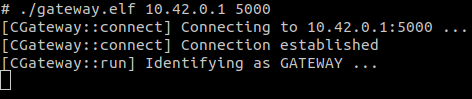
\includegraphics[width=.76\textwidth]{13tests/gateway/GatewayConnect}
	\caption{Test Gateway: Connection to RS.}
	\label{fig:}
\end{figure}

When the remote system acknowledges the connection from the gateway, it will answer to the connection request of a local system (\verb|CRQ|) with a new ID. In figure \ref{fig:recvMin} one can see that, the gateway receives the \verb|CRQ| command using \verb|LoRa|. When the remote system answers, the gateway receives the message using \verb|TCP|. It is also visible that the command \verb|CRQ| sent by the local system, is converted in \verb|CRQ;<addr>|, as well as the command sent from the remote system \verb|ID;<id>;<addr>| is converted to \verb|ID;<id>|, where the destination field on the LoRa message is the specified \verb|<addr>|.

\begin{figure}[H]
	\centering	
	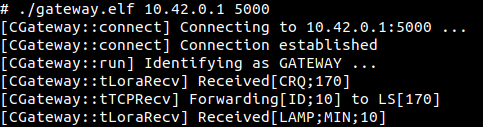
\includegraphics[width=.76\textwidth]{13tests/gateway/recvMin}
	\caption{Test Gateway: Receiving commands from the LS.}
	\label{fig:recvMin}
\end{figure}

%**********************************************************
\clearpage
\section{Website}
In order to validate that the website is correctly reading all parking spaces information from the database, one can see the result of fetching info from the database before and after inserting a parking space into the database.

In listing \ref{lst:testwebsite} is presented the queries needed to insert a parking space which is linked to a lamppost and to a location. In line 9 one defines the number of vacants at 3.

\begin{lstlisting}[language=SQL, caption={Test Website: add parking space to the database.}, label={lst:testwebsite}]
INSERT INTO region(post_code, operator_id, parish, county, district) 
	VALUES('4800-073', 2, 'Azurem', 'Guimaraes', 'Braga');

INSERT INTO location(id, latitude, longitude, post_code, street_name) 
	VALUES(1, 41.447849, -8.298462, '4800-073', 'Rua Teixeira de Pascoais');

INSERT INTO lamppost(id, address) VALUES (1, 0xa2);

UPDATE parking_space SET num_vacants=3 WHERE id=1;
\end{lstlisting}

Below one can see the result in the website, before and after the insertion of the parking space.

\begin{figure}[H]
	\centering
	\begin{subfigure}{.4\textwidth}
		\centering
		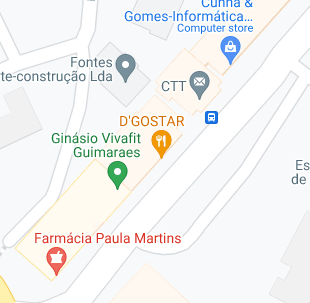
\includegraphics[width=.95\linewidth]{13tests/website/beforeinsert}
		\caption{Before parking space insert.}
		\label{fig:login}
	\end{subfigure}%
	\begin{subfigure}{.4\textwidth}
		\centering
		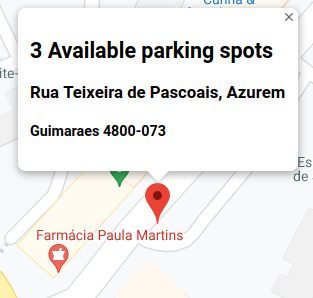
\includegraphics[width=.95\linewidth]{13tests/website/afterinsert}
		\caption{After parking space insert.}
		\label{fig:menu}
	\end{subfigure}
	\caption{Test website.}
	\label{fig:applogin}
\end{figure}

%**********************************************************
\clearpage
\section{Mobile Application}

To test the mobile application, the remote server was started in the machine with IP \verb|192.168.1.114|. After connecting to the remote server, the operator can login in the application. In figure \ref{fig:applogin}, one can see that, after inserting the correct credentials, the application menu appears, showing that the login process was successfully done.

\begin{figure}[H]
	\centering
	\begin{subfigure}{.4\textwidth}
		\centering
		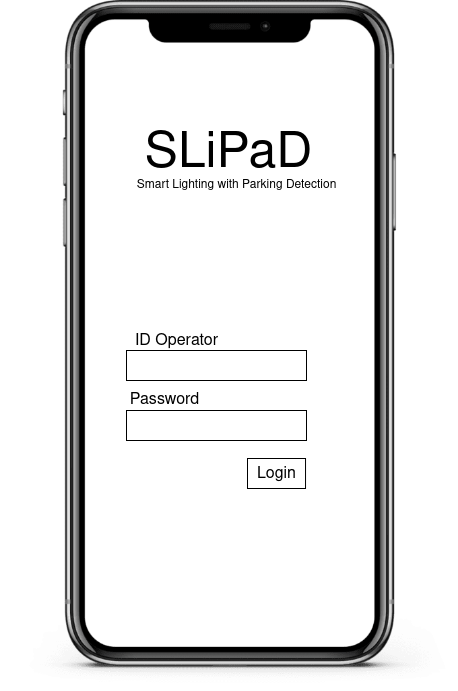
\includegraphics[width=.95\linewidth]{13tests/app/login}
		\caption{Login.}
		\label{fig:login}
	\end{subfigure}%
	\begin{subfigure}{.4\textwidth}
		\centering
		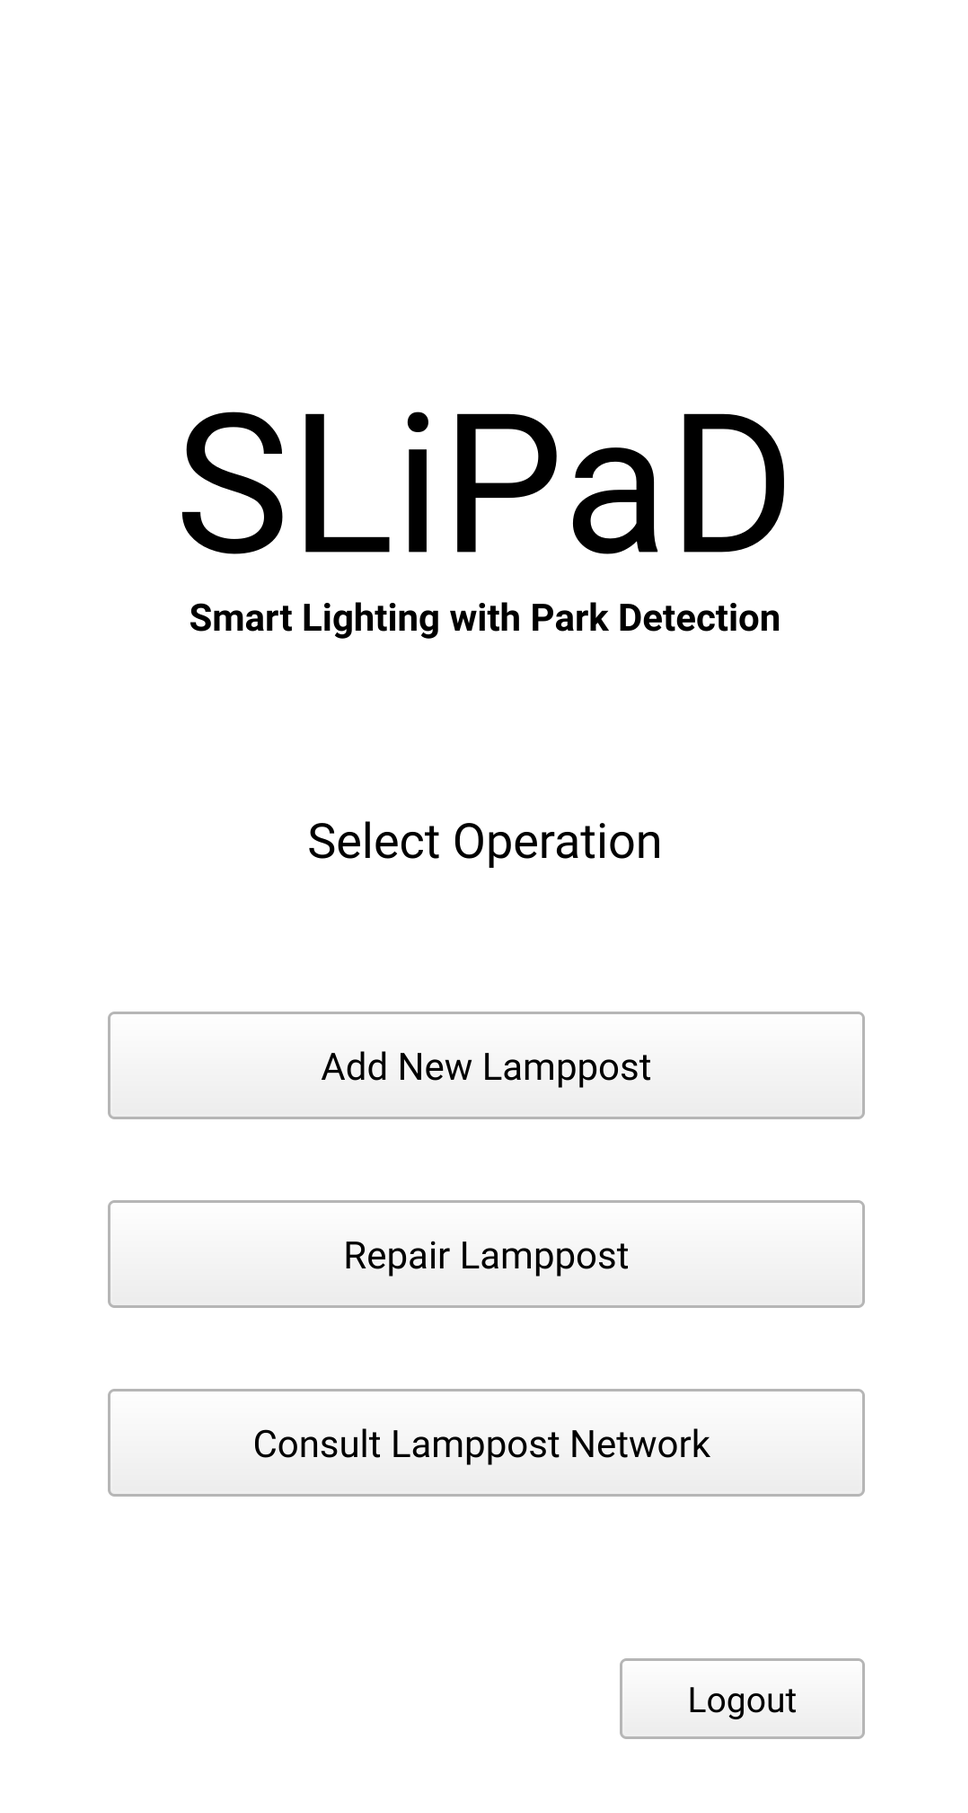
\includegraphics[width=.95\linewidth]{13tests/app/menu}
		\caption{Menu.}
		\label{fig:menu}
	\end{subfigure}
	\caption{Mobile Application Login Process.}
	\label{fig:applogin}
\end{figure}

If the credentials were wrong, the message presented in figure \ref{fig:login_wrong} is shown, and the login fails. Furthermore, if any operation performed by the operator fails, the application shows an error message.

\begin{figure}[H]
	\centering	
	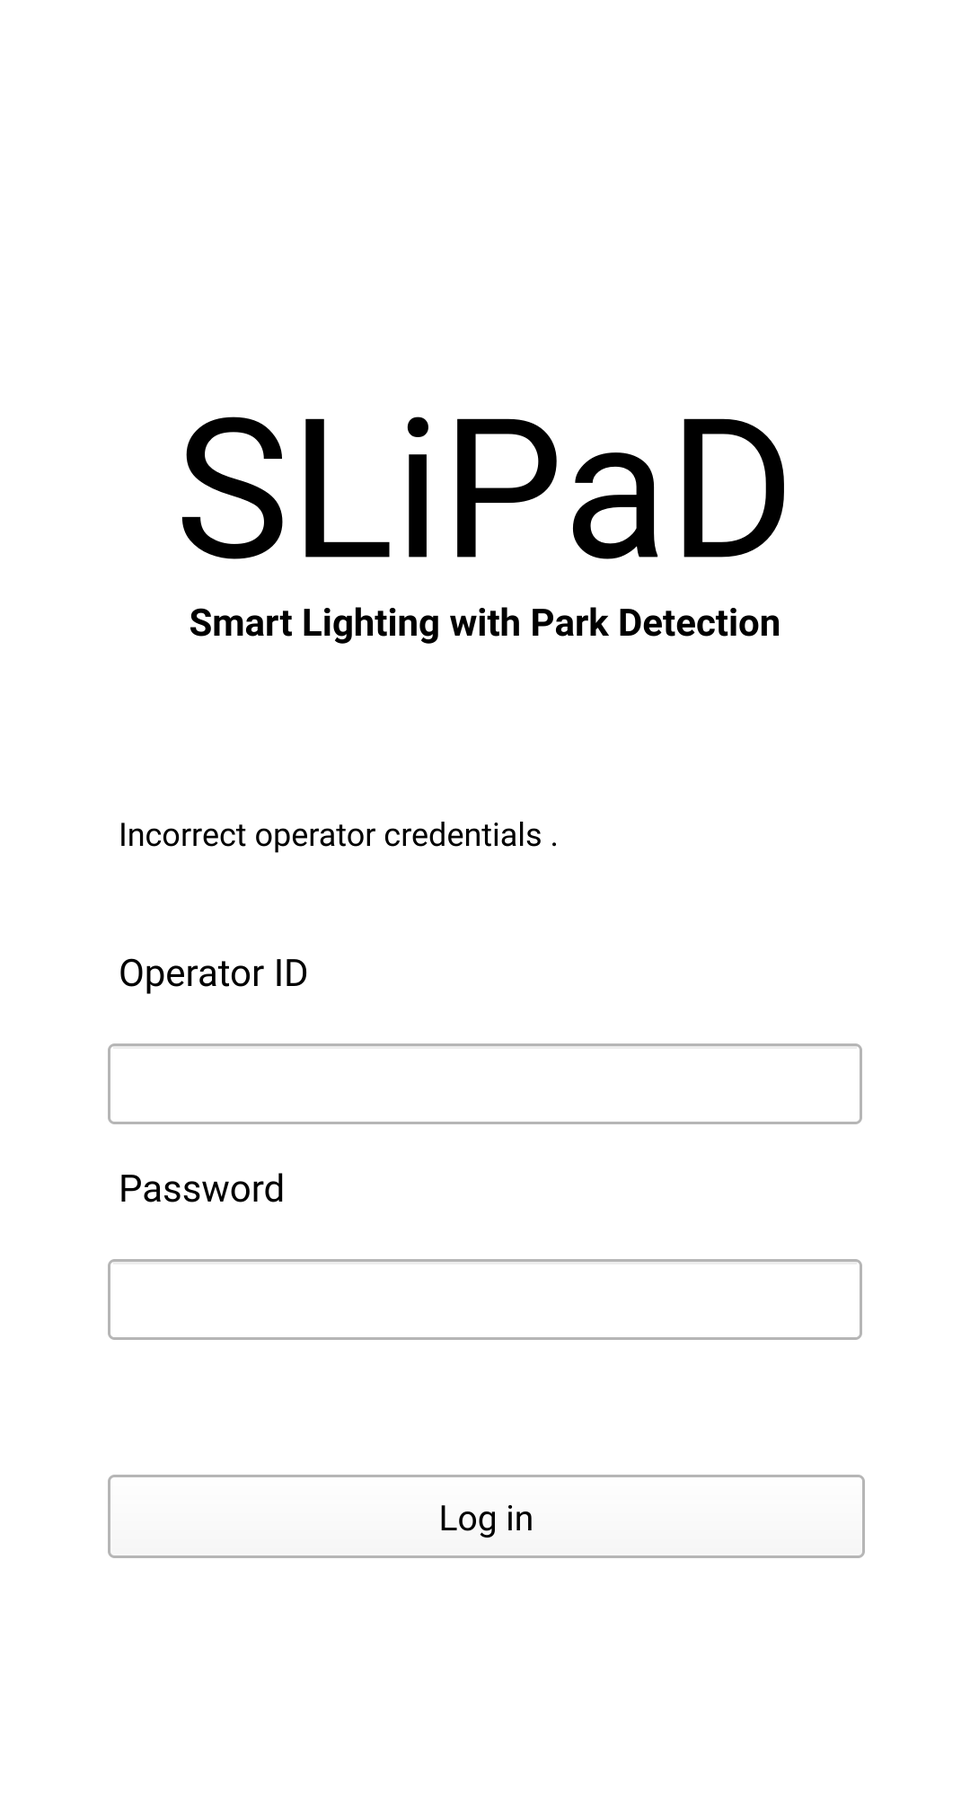
\includegraphics[width=.4\textwidth]{13tests/app/login_wrong}
	\caption{Test Mobile Application: Test login - Wrong credentials.}
	\label{fig:login_wrong}
\end{figure}

When the operator selects \verb|Consult Lamppost Network|, the mobile application sends a request for the remote server and receive all the lamppost information relative to that operator. In figure \ref{fig:consult}, one can observed the lamppost network information relative to the operator with ID number 2.

\begin{figure}[H]
	\centering	
	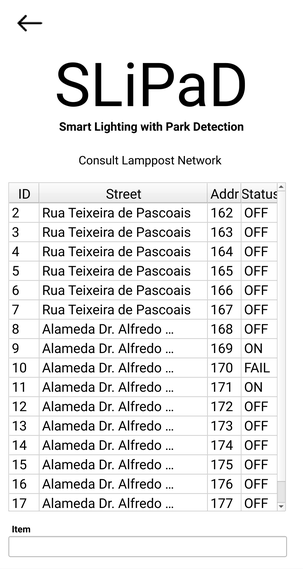
\includegraphics[width=.4\textwidth]{13tests/app/consult}
	\caption{Test Mobile Application: Consult lamppost network.}
	\label{fig:consult}
\end{figure}

%**********************************************************
\section{Remote System}

Regarding Remote Systems tests, one recorded a video (available on \linebreak \url{https://youtu.be/KpZ--wc1S-c}) demonstrating the connection between the local system's parking detection, and the remote system's website.

In figure \ref{fig:rsnewgateway} is shown the process of connecting a gateway to the remote system. Initially, the remote system is put to run, having its TCP server listening for incoming connections on port \verb|5000|, on socket file descriptor 3. When a new client connects via TCP it needs to send the \verb|TYPE;<clientType>| command. This command is used by any of the remote clients (gateway or mobile application) and identifies which type of remote client the new client is. If the received type, \verb|<clientType>|, equals 0, as shown in the figure, then the remote client trying to connect is a gateway.

\begin{figure}[H]
	\centering	
	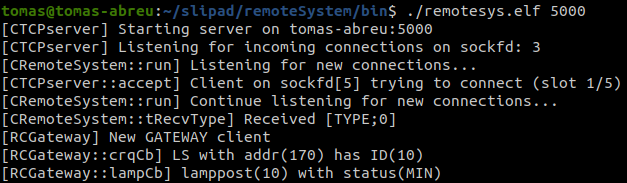
\includegraphics[width=.76\textwidth]{13tests/RS/RSsendID}
	\caption{Test Remote System: New gateway connection.}
	\label{fig:rsnewgateway}
\end{figure}

After connection between gateway and remote system has been established, the local system sends the \verb|CRQ;<localAddr>| command, regarding a connection request. This command is an handshake from the two systems, where the remote system gives to the local system a new ID. The local system, from now on, uses the given ID in all communications.

In figure \ref{fig:RScmdsfromLS} is shown the receival of local system's commands. It is visible that after the \verb|CRQ| command, where a local system with address 170 receives an ID of 10, the communications are made using that ID, in \verb|lamppost(10)|. Firstly, one can see the lamppost changing its status to \verb|MIN|. When the lamppost changes its status to \verb|ON|, the remote system must determine which lampposts should also turn on, executing a dynamic light up of the network lampposts. As a proof of concept, the remote system considers the neighbour lampposts as the ones with the ID above and below of the ID of the lamppost that turned on. For that reason, one can see that when \verb|lamppost(10)| turns on, the remote system requests \verb|lamppost(9)| and \verb|lamppost(11)| to turn on their lamp.

\begin{figure}[H]
	\centering	
	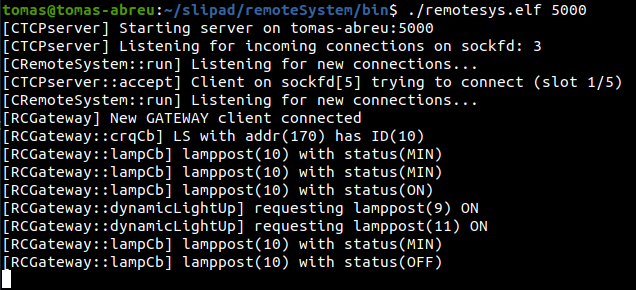
\includegraphics[width=.7\textwidth]{13tests/RS/RScmdsfromLS}
	\caption{Test Remote System: Dynamic control of lamps.}
	\label{fig:RScmdsfromLS}
\end{figure}

In figure \ref{fig:RSpark} is shown the remote system output of when receiving \linebreak \verb|PARK;<numVacants>| command. This information is updated on the database, allowing the fetch from the website to retrieve the most updated network information, which will be detailed in the following section.

\begin{figure}[H]
	\centering	
	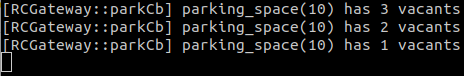
\includegraphics[width=.7\textwidth]{13tests/RS/RSpark}
	\caption{Test Remote System: Parking space detection from LS.}
	\label{fig:RSpark}
\end{figure}

Regarding a mobile application remote client, the procedure for identifying the remote client is equal to the gateway. In figure \ref{fig:RScmdsApp} one can see the output of mobile application operations: signing in, adding a lamppost - which demands inserting a region, if this doesn't exist in the system, inserting a location, and finally the lamppost - and consulting the lampposts list that the operator signed in is in charge.

\begin{figure}[H]
	\centering	
	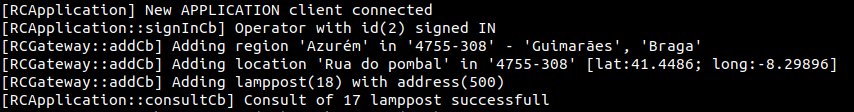
\includegraphics[width=1\textwidth]{13tests/RS/RScmdsApp}
	\caption{Test Remote System: New mobile application connection.}
	\label{fig:RScmdsApp}
\end{figure}

In figure \ref{fig:RSrepairApp} is shown the output of the mobile application using the repair funcionality. A lamppost with status \verb|FAIL| can be repaired by the operator, having its state back to \verb|OFF|, if the repair was made during the day, or back to \verb|MIN|, if the repair was made late in the afternoon, and the local system has already detected low luminosity conditions.

\begin{figure}[H]
	\centering	
	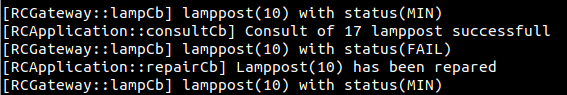
\includegraphics[width=.7\textwidth]{13tests/RS/RSrepairApp}
	\caption{Test Remote System: Application repair command.}
	\label{fig:RSrepairApp}
\end{figure}
